% \begin{document}
\section{Matroid Intersection}

Although the concept of matroids forms a rich set of problems that can be solved by the greedy
algorithm, there are many problems that have efficient algorithms but are not matroids. Consider
for example the bipartite matching problem:

\dfn{Max Size Matching}{\label{def:bm}
Given a bipartite graph $G=(V,E)$, find a matching of maximum size.
}

Recall that a matching $M\subseteq E$ is a subset of edges so that every vertex is incident to at
most one edge of $M$, i.e., $|\{e\in M: v\in e\}|\le 1$ for all $v\in V$.

\ex{}{
The edges $(1,4)$ and $(3,5)$ form a matching (of maximum cardinality).

\begin{center}
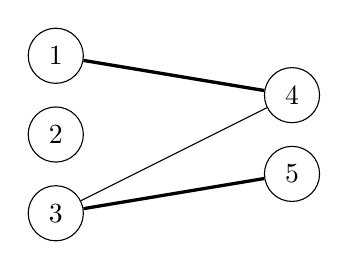
\begin{tikzpicture}[every node/.style={circle,draw,minimum size=7mm,inner sep=0pt}]
  \node (1) at (0,2) {1};
  \node (2) at (0,1) {2};
  \node (3) at (0,0) {3};
  \node (4) at (3,1.5) {4};
  \node (5) at (3,0.5) {5};
  \draw[very thick] (1) -- (4);
  \draw (3) -- (4);
  \draw[very thick] (3) -- (5);
\end{tikzpicture}
\end{center}
}

Let's see if \Greedy{} works for maximum cardinality (or max weight) bipartite matching. To do
this, we can verify if $(E,\I)$ is a matroid where
\[
  \I=\{M\subseteq E: M \text{ is a matching}\}.
\]
It is easy to see that $(E,\I)$ satisfies the downward closed property (I1) of matroids since a
subset of a matching is still a matching. However, the second axiom (I2) is not satisfied which
can be seen by taking the two matchings $M_1=\{(1,4),(3,5)\}$ and $M_2=\{(3,4)\}$: although
$|M_1|>|M_2|$ there is no edge in $M_1$ that we can add to $M_2$ while maintaining that it is a
matching.

This is kind of sad: matroids and simple \Greedy{} have their limits. On the other hand, we know
from our undergraduate algorithm course that there are efficient algorithms for the bipartite
matching problem. That there are efficient algorithms for the bipartite matching problem is in
fact part of a more general phenomena: it can be described as the intersection of two matroids
and any such problem has an efficient algorithm!

\dfn{Matroid Intersection}{
Given two matroids $\M_1=(E,\I_1)$ and $\M_2=(E,\I_2)$ on the same ground set $E$, their
intersection is
\[
  \M_1\cap\M_2=(E,\I_1\cap\I_2).
\]
}

Note that the intersection of two matroids satisfy (I1) but not typically (I2). The following adds
a lot of power to the concepts of matroids:

\thm{Edmonds, Lawler, 70's}{\label{thm:edmonds}
There is an efficient algorithm for finding a max-weight independent set in the intersection of
two matroids.\footnote{It is efficient meaning that it is a polynomial-time algorithm if we can,
in polynomial time, answer independence queries of the type ``$I\in\I_1$?'' and ``$I\in\I_2$?''
for the two matroids (which is the case for all examples of matroids seen in class).}
}

The algorithm that gives the above result is quite technical and notation heavy. Instead of
describing it in its full generality, we first see how we can apply the above result to obtain
several interesting algorithmic applications. We then develop an algorithm for the special case of
the bipartite matching problem that share several similarities with the general algorithm.

\subsection{Examples}

From \url{http://www-math.mit.edu/~goemans/18433S09/matroid-intersect-notes.pdf}

\subsubsection{Bipartite Matching}

We already mentioned that the bipartite matching problem is an example of matroid intersection.
To see this, consider a bipartite graph $G=(V,E)$ with bipartition $(A,B)$.

Let $\M_A$ be a partition matroid with ground set $E$ where the partition $E$ is given by
$E=\bigcup\{\delta(v): v\in A\}$ where $\delta(v)$ denotes the edges incident to $v$. Notice that
this is a partition since all edges have precisely one endpoint in $A$. We also define $k_v=1$ for
every $v\in A$. Thus, the family of independent sets of $\M_A$ is given by
\[
  \I_A=\{F\subseteq E: |F\cap\delta(v)|\le 1 \text{ for all } v\in A\}.
\]
In other words, a set of edges is independent for $\M_A$ if it has at most one edge incident to
every vertex of $A$ (and any number of edges incident to every vertex of $B$). We can similarly
define $\M_B=(E,\I_B)$ by
\[
  \I_B=\{F\subseteq E: |F\cap\delta(v)|\le 1 \text{ for all } v\in B\}.
\]
Now observe that any $F\in\I_A\cap\I_B$ corresponds to a matching in $G$, and vice versa. And the
largest common independent set $\I_A$ and $\I_B$ corresponds to a maximum matching in $G$.

\subsubsection{Colorful Spanning Trees}

Suppose we have an undirected graph $G=(V,E)$ and every edge has a color. This is represented by a
partition of $E$ into $E_1\cup E_2\cup\cdots\cup E_k$ where each $E_i$ represents a set of edges
of the same color $i$. The problem of deciding whether this graph has a spanning tree in which all
edges have a different color can be tackled through matroid intersection. Such a spanning tree is
called \emph{colorful}. Colorful spanning trees are bases of the graphic matroid
$\M_1=(E,\I_1)$ of $G$ which are also independent in the partition matroid $\M_2=(E,\I_2)$
defined by $\I_2=\{F\subseteq E: |F\cap E_i|\le 1 \text{ for all } i\}$.

\subsubsection{Arborescences}

Given a directed graph $D=(V,A)$ and a special root vertex $r\in V$, an \emph{$r$-arborescence}
(or just arborescence) is a spanning tree (when viewed as an undirected graph) directed away from
$r$. Thus, in a $r$-arborescence, every vertex is reachable from the root $r$. As an
$r$-arborescence has no arc incoming to the root, we assume that $D$ has no such arc.

\ex{}{
The following directed graph has e.g.\ the $r$-arborescence $\{(r,B),(B,C),(B,D)\}$.

\begin{center}
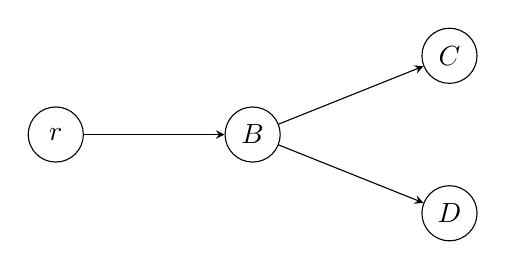
\begin{tikzpicture}[every node/.style={circle,draw,minimum size=7mm,inner sep=0pt},
                    >=stealth]
  \node (r) at (0,0) {$r$};
  \node (B) at (2.5,0) {$B$};
  \node (C) at (5,1) {$C$};
  \node (D) at (5,-1) {$D$};
  \draw[->] (r) -- (B);
  \draw[->] (B) -- (C);
  \draw[->] (B) -- (D);
\end{tikzpicture}
\end{center}
}

$r$-arborescences can be viewed as sets simultaneously independent in two matroids. Let $G$ denote
the undirected counterpart of $D$ obtained by disregarding the directions of the arcs. Note that
if we have both arcs $a_1=(u,v)$ and $a_2=(v,u)$ in $D$ then we get two undirected edges also
labeled $a_1$ and $a_2$ between $u$ and $v$ in $G$. Define $\M_1=(A,\I_1)$ the graphic matroid
corresponding to $G$, and $\M_2=(A,\I_2)$ the partition matroid in which independent sets are
those with at most one arc incoming to every vertex $v\neq r$. In other words, we let
\[
  \I_2=\{F: |F\cap\delta^-(v)|\le 1 \text{ for all } v\in V\setminus\{r\}\},
\]
where $\delta^-(v)$ denotes the set $\{(u,v)\in A\}$ of arcs incoming to $v$. Thus, any
$r$-arborescence is independent in both matroids $\M_1$ and $\M_2$. Conversely, any set $T$
independent in both $\M_1$ and $\M_2$ and of cardinality $|V|-1$ (so that it is a base in both
matroids) is an $r$-arborescence. Indeed, such a $T$ being a spanning tree in $G$ has a unique path
between $r$ and any vertex $v$; this path must be directed from the root $r$ since otherwise we
would have either an arc incoming to $r$ or two arcs incoming to the same vertex.
% \end{document}
